
\begin{figure}[H]
  \centering
  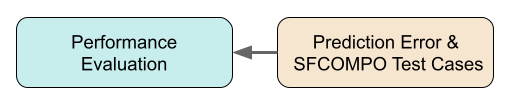
\includegraphics[width=0.7\linewidth]{./chapters/exp1/methodology4.png}
  \caption{Fourth portion of the flowchart from Figure \ref{fig:method} being 
           described in this section.}
\end{figure}

\subsection{Random Error Impacts on Prediction}
\label{sec:randerr}

\begin{figure}[!ht]
    \centering
    \begin{subfigure}[b]{0.49\textwidth}
        \centering
        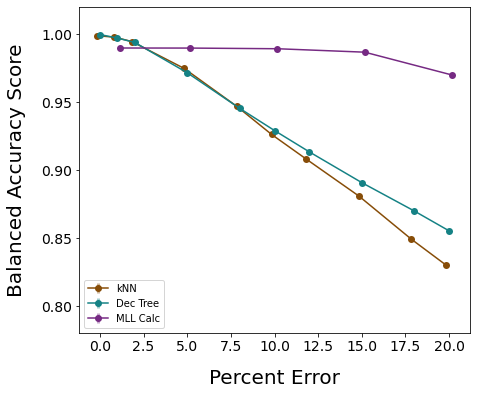
\includegraphics[width=\textwidth]{./chapters/exp1/randerr_compare_nuc29_BalAcc_rxtr.png}
        \caption{Balanced accuracy of reactor type classification.}
        \label{fig:randerrA}
    \end{subfigure}
    \hfill
    \begin{subfigure}[b]{0.49\textwidth}
        \centering
        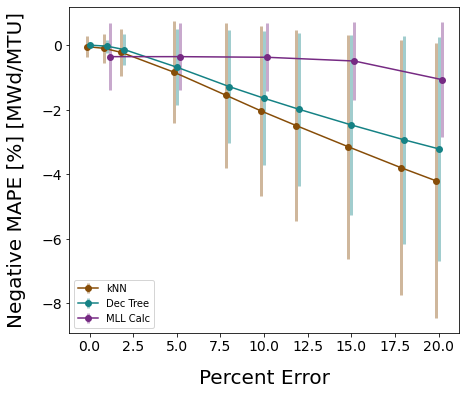
\includegraphics[width=\textwidth]{./chapters/exp1/randerr_compare_nuc29_MAPE_burn.png}
        \caption{Negative \gls{MAPE} of burnup regression.}
        \label{fig:randerrB}
    \end{subfigure}
    \vskip\baselineskip
    \begin{subfigure}[b]{0.49\textwidth}
        \centering
        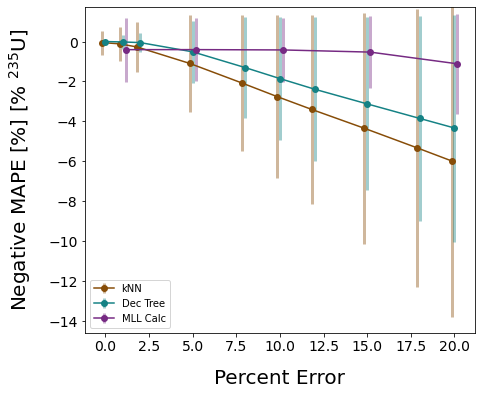
\includegraphics[width=\textwidth]{./chapters/exp1/randerr_compare_nuc29_MAPE_enri.png}
        \caption{Negative \gls{MAPE} of \gls{U235} regression.}
        \label{fig:randerrC}
    \end{subfigure}
    \hfill
    \begin{subfigure}[b]{0.49\textwidth}
        \centering
        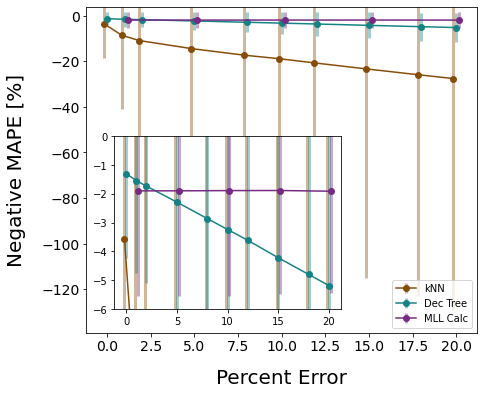
\includegraphics[width=\textwidth]{./chapters/exp1/randerr_compare_nuc29_MAPE_cool.png}
        \caption{Negative \gls{MAPE} of time since irradiation regression.} 
        \label{fig:randerrD}
    \end{subfigure}
    \caption{Prediction performance with respect to decreasing information
             quality in the form of uniform/random error applied to the nuclide 
             mass measurements in the training set.}
    \label{fig:randerr}
\end{figure}

As previously introduced in Section \ref{sec:testerr}, the prediction
performance is measured by evaluating the accuracy of the reactor type
classification or the error of the regression cases (burnup, \gls{U235}
enrichment, cooling time).  These performance metrics for all four prediction
types are compared across the three algorithms used: \textit{k}-nearest
neighbors (denoted in plots as \textit{kNN}), decision trees (denoted in plots
as \textit{Dec Tree} or \textit{DTree}), and \gls{MLL} calculations.  To judge
the degradation of predictions of the algorithms with increasing nuclide mass
measurement error (i.e., reduced information quality, detailed in section
\ref{sec:inforeduc1}), four plots are made with the introduced error on the
\textit{x}-axis and a prediction performance metric on the \textit{y}-axis.
Shown in Figure \ref{fig:randerr}, the \textit{y}-axis is always oriented so
that lower is poorer performance and higher is better performance. This is why
Figures \ref{fig:randerrB}--\ref{fig:randerrD} present a negative error on the
\textit{y}-axis.
\todo[inline]{In order to have consistency in plot presentation w future plots,
the plots in this section have a small delta-x to show error bars that are
otherwise hard to see.  Since the x-axis is continuous, this may force a return
to using the fill-between to visualize error bands instead.}

Figure \ref{fig:randerrA} shows the balanced accuracy of reactor type
classification, where a score of $1$ is perfect prediction and a score of $0$
is random classification. The error bars reflect a 99\% confidence interval.
While the two scikit-learn algorithms follow a very similar path of decreased
accuracy as the error increases, the \gls{MLL} calculation approach appears to
be more robust to the nuclide mass measurement error. This behavior is seen in
all four plots in Figure \ref{fig:randerr}. Another interesting result is that
the \gls{MLL} calculation performs slightly worse for low errors. If the
expected measurement errors of nuclide masses in a training database or in a
test sample can be guaranteed to be better than ~2\%, the \gls{MLL} calculation
is no longer the obvious preferred choice for reactor type prediction.

Figure \ref{fig:randerrB} demonstrates the first regression performance plot.
As mentioned, the \textit{x}-axis is negative \gls{MAPE} so that higher is
always better.  The error bars reflect one standard deviation of the average
percentage errors.  Again, the \gls{MLL} method is robust to training set error
but performs slightly worse at low error values.  All three methods calculate
burnup with a maximum error of 5\% at 20\% error in the training set.  While it
is difficult to draw an acceptable baseline, this minimum performance level can
serve as a benchmark for the work presented in Chapter \ref{ch:exp2}. 

Figure \ref{fig:randerrC}

is about 6\%. The error bars reflect one standard deviation of the 
average percentage errors.

the maximum error of \textit{k}-nearest neighbors reaches nearly 
30\%, but the other two are under 10\% error. The error bars 
reflect one standard deviation of the average percentage errors.


\begin{figure}[!ht]
    \centering
    \begin{subfigure}[b]{\textwidth}
        \centering
        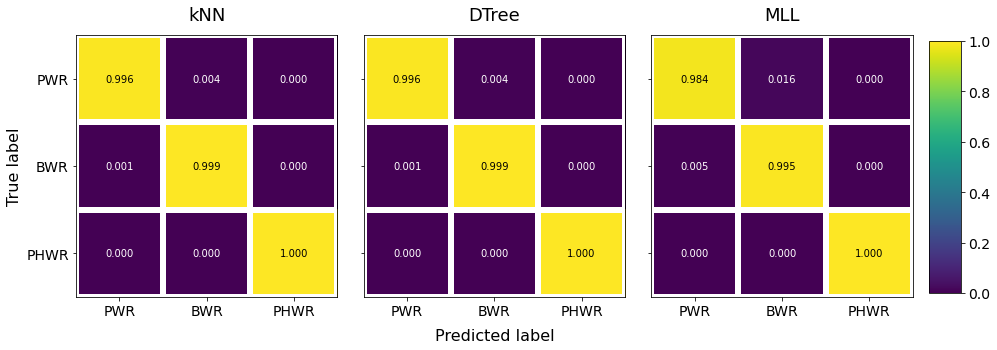
\includegraphics[width=\textwidth]{./chapters/exp1/confusion_matrix_nuc29_err01.png}
        \caption[]{1\% error}
        %\label{fig:}
    \end{subfigure}
    \vskip\baselineskip
    \begin{subfigure}[b]{\textwidth}
        \centering
        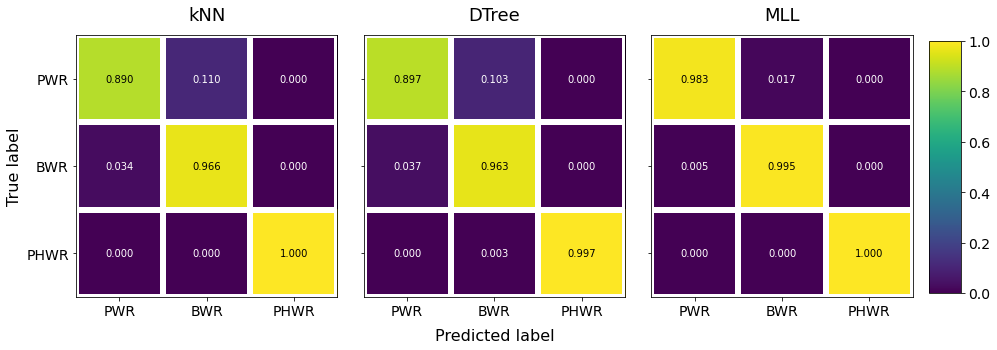
\includegraphics[width=\textwidth]{./chapters/exp1/confusion_matrix_nuc29_err10.png}
        \caption[]{10\% error}
        %\label{fig:}
    \end{subfigure}
    \caption[]{Confusion matrices for reactor type prediction, two different error injection levels.}
    \label{fig:cm_nuc29}
\end{figure}

\begin{figure}[!ht]
    \centering
    \begin{subfigure}[b]{0.49\textwidth}
        \centering
        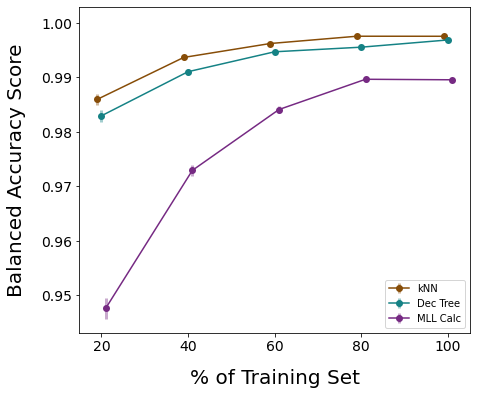
\includegraphics[width=\textwidth]{./chapters/exp1/learncurve_nuc29_BalAcc_rxtr.png}
        \caption[]{Caption.}
        %\label{fig:}
    \end{subfigure}
    \hfill
    \begin{subfigure}[b]{0.49\textwidth}
        \centering
        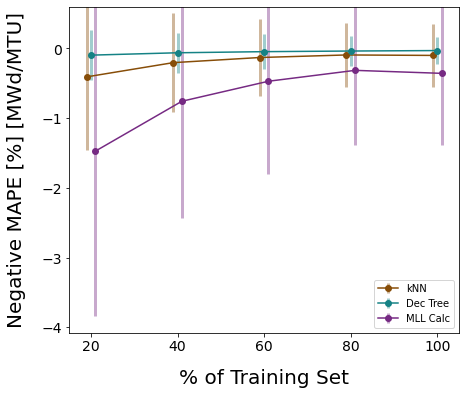
\includegraphics[width=\textwidth]{./chapters/exp1/learncurve_nuc29_MAPE_burn.png}
        \caption[]{Caption.}
        %\label{fig:}
    \end{subfigure}
    \vskip\baselineskip
    \begin{subfigure}[b]{0.49\textwidth}
        \centering
        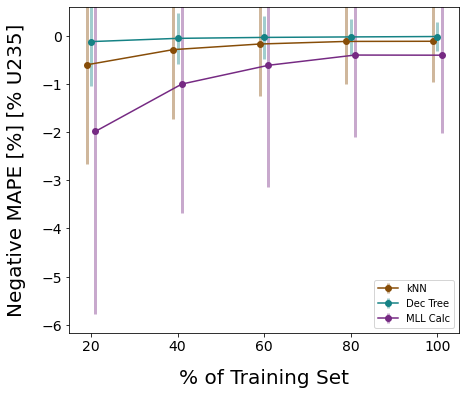
\includegraphics[width=\textwidth]{./chapters/exp1/learncurve_nuc29_MAPE_enri.png}
        \caption[]{Caption.}
        %\label{fig:}
    \end{subfigure}
    \hfill
    \begin{subfigure}[b]{0.49\textwidth}
        \centering
        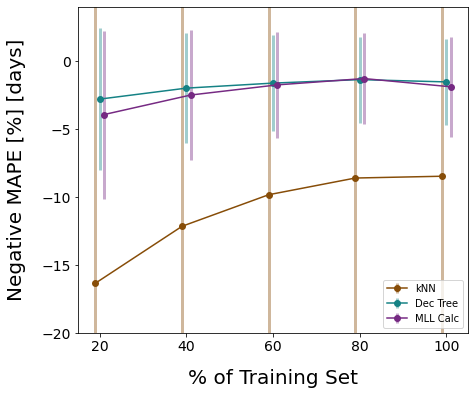
\includegraphics[width=\textwidth]{./chapters/exp1/learncurve_nuc29_MAPE_cool.png}
        \caption[]{Caption.}
        %\label{fig:}
    \end{subfigure}
    \caption[]{Learning curves.}
    \label{fig:learns}
\end{figure}

\begin{figure}[!ht]
  \centering
  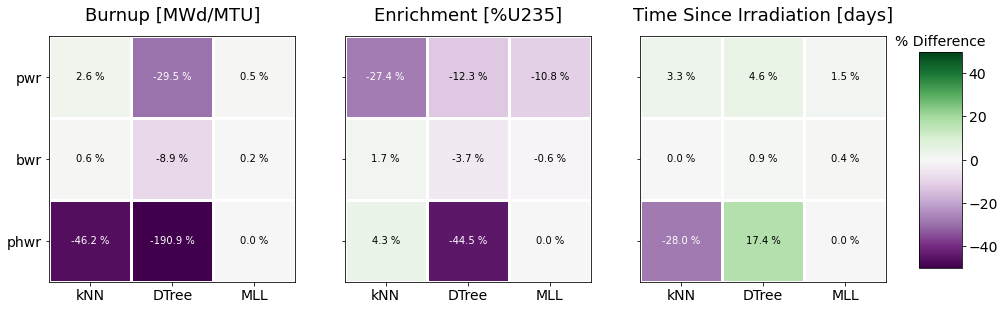
\includegraphics[width=1.1\textwidth]{./chapters/exp1/rxtr-type_known-unknown_diff.png}
  \caption{diff.}
  \label{fig:knownrxtr}
\end{figure}

\subsection{SFCOMPO Test Set}
\label{sec:sfcompo}

The testing described in Section \ref{sec:randerr} describes the process of
evaluating the methodology with test cases drawn from the training database.
It is also helpful to test the methodology against real assays of \gls{SNF}.
The \gls{SFCOMPO} database was created to allow access to these sorts of
measurements linked to the reactor operation parameters being predicted in this
work. The only parameter not part of the \gls{SFCOMPO} database is the time
since irradiation, so that is not predicted here. 

There are 505 test cases that are able to be compared against the training
database.  The number of each reactor type is as follows: 312 \gls{PWR}s, 165
\gls{BWR}s, and 28 \gls{PHWR}s. The space of enrichment and burnup values is
visualized in Figure \ref{fig:sfcoscatter}. These are sufficienty represented
in the training set design, as pictured in Figure \ref{fig:trainhist}.

\begin{figure}[!ht]
    \centering
    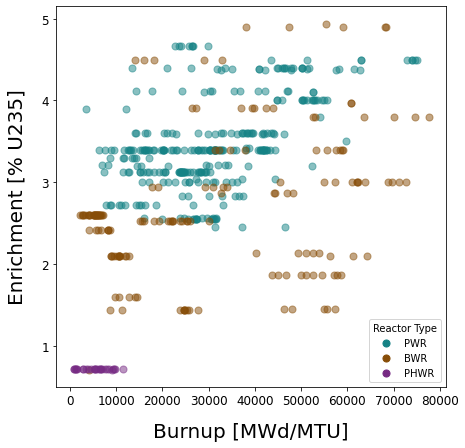
\includegraphics[width=0.7\textwidth]{./chapters/exp1/sfcompo_scatter_viz.png}
    \caption{Scatter plot showing the range of reactor operation parameters in 
             the \gls{SFCOMPO} testing set that are being predicted.}
    \label{fig:sfcoscatter}
    \todo[inline]{increase tick size, change order to bwr, pwr, phwr. Maybe show 
                  comparison against training E v B scatter plot}
\end{figure}



\begin{table}[!ht]
  \centering
  \begin{tabular}{@{}l|lll|lll@{}}
  \toprule
                   & \multicolumn{3}{l|}{Accuracy Scores} & \multicolumn{3}{l}{Balanced Accuracy Scores} \\ \toprule
  Null Handling    & kNN        & DTree      & MLL       & kNN           & DTree         & MLL           \\ \midrule
  Imputed Nulls    & 0.52       & 0.60       & 0.39      & 0.09          & 0.12          & 0.00          \\
  Zero-value Nulls & 0.45       & 0.42       & 0.72      & 0.21          & 0.30          & 0.63          \\ \bottomrule
  \end{tabular}
  \caption{sfcompo reactor accuracies.}
  \label{tbl:sfcorxtr}
\end{table}

\begin{figure}[!ht]
    \centering
    \begin{subfigure}[b]{0.49\textwidth}
        \centering
        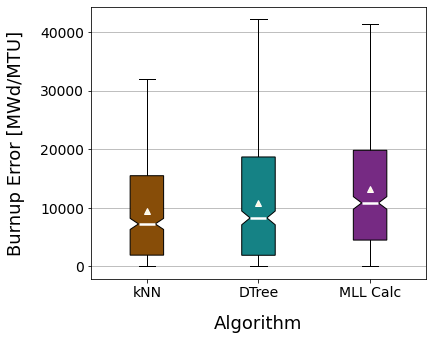
\includegraphics[width=\textwidth]{./chapters/exp1/sfcompo_boxplots_impnull_burn.png}
        \caption[]{Caption.}
        %\label{fig:}
    \end{subfigure}
    \hfill
    \begin{subfigure}[b]{0.49\textwidth}
        \centering
        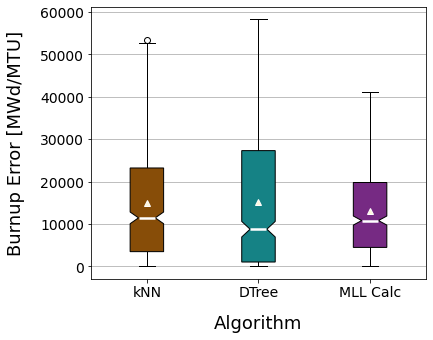
\includegraphics[width=\textwidth]{./chapters/exp1/sfcompo_boxplots_0null_burn.png}
        \caption[]{Caption.}
        %\label{fig:}
    \end{subfigure}
    \caption{sfcompo burnup boxplots.}
    \label{fig:sfcoburn}
\end{figure}

\begin{table}[!ht]
  \centering
  \begin{tabular}{@{}l|lll|lll@{}}
  \toprule
                   & \multicolumn{3}{l|}{Mean Errors [GWd/MTU]} & \multicolumn{3}{l}{Median Errors [GWd/MTU]} \\ \toprule
  Null Handling    & kNN           & DTree         & MLL           & kNN            & DTree          & MLL    \\ \midrule
  Imputed Nulls    & 9.43          & 10.89         & 13.17         & 7.26           & 8.28           & 10.84  \\
  Zero-value Nulls & 14.88         & 15.18         & 3.53          & 11.47          & 8.79           & 1.70   \\ \bottomrule
  \end{tabular}
  \caption{sfcompo burnup errors.}
  \label{tbl:sfcoburn}
\end{table}

\begin{figure}[!ht]
    \centering
    \begin{subfigure}[b]{0.49\textwidth}
        \centering
        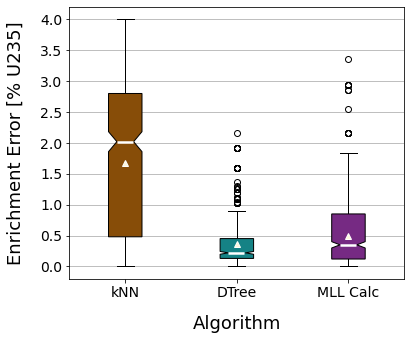
\includegraphics[width=\textwidth]{./chapters/exp1/sfcompo_boxplots_0null_enri.png}
        \caption[]{Caption.}
        %\label{fig:}
    \end{subfigure}
    \hfill
    \begin{subfigure}[b]{0.49\textwidth}
        \centering
        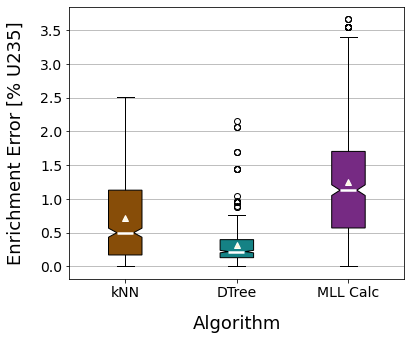
\includegraphics[width=\textwidth]{./chapters/exp1/sfcompo_boxplots_impnull_enri.png}
        \caption[]{Caption.}
        %\label{fig:}
    \end{subfigure}
    \caption{sfcompo enrichment boxplots.}
    \label{fig:sfcoenri}
\end{figure}

\begin{table}[!ht]
  \centering
  \begin{tabular}{@{}l|lll|lll@{}}
  \toprule
                   & \multicolumn{3}{l|}{Mean Errors [\% U235]} & \multicolumn{3}{l}{Median Errors [\% U235]} \\ \toprule
  Null Handling    & kNN           & DTree          & MLL          & kNN            & DTree          & MLL    \\ \midrule
  Imputed Nulls    & 0.72          & 0.31           & 1.25         & 0.50           & 0.22           & 1.13   \\
  Zero-value Nulls & 1.67          & 0.36           & 0.49         & 2.02           & 0.22           & 0.35   \\ \bottomrule
  \end{tabular}
  \caption{sfcompo enrichment errors.}
  \label{tbl:sfcoenri}
\end{table}

